\begin{figure}[h!]
\begin{center}
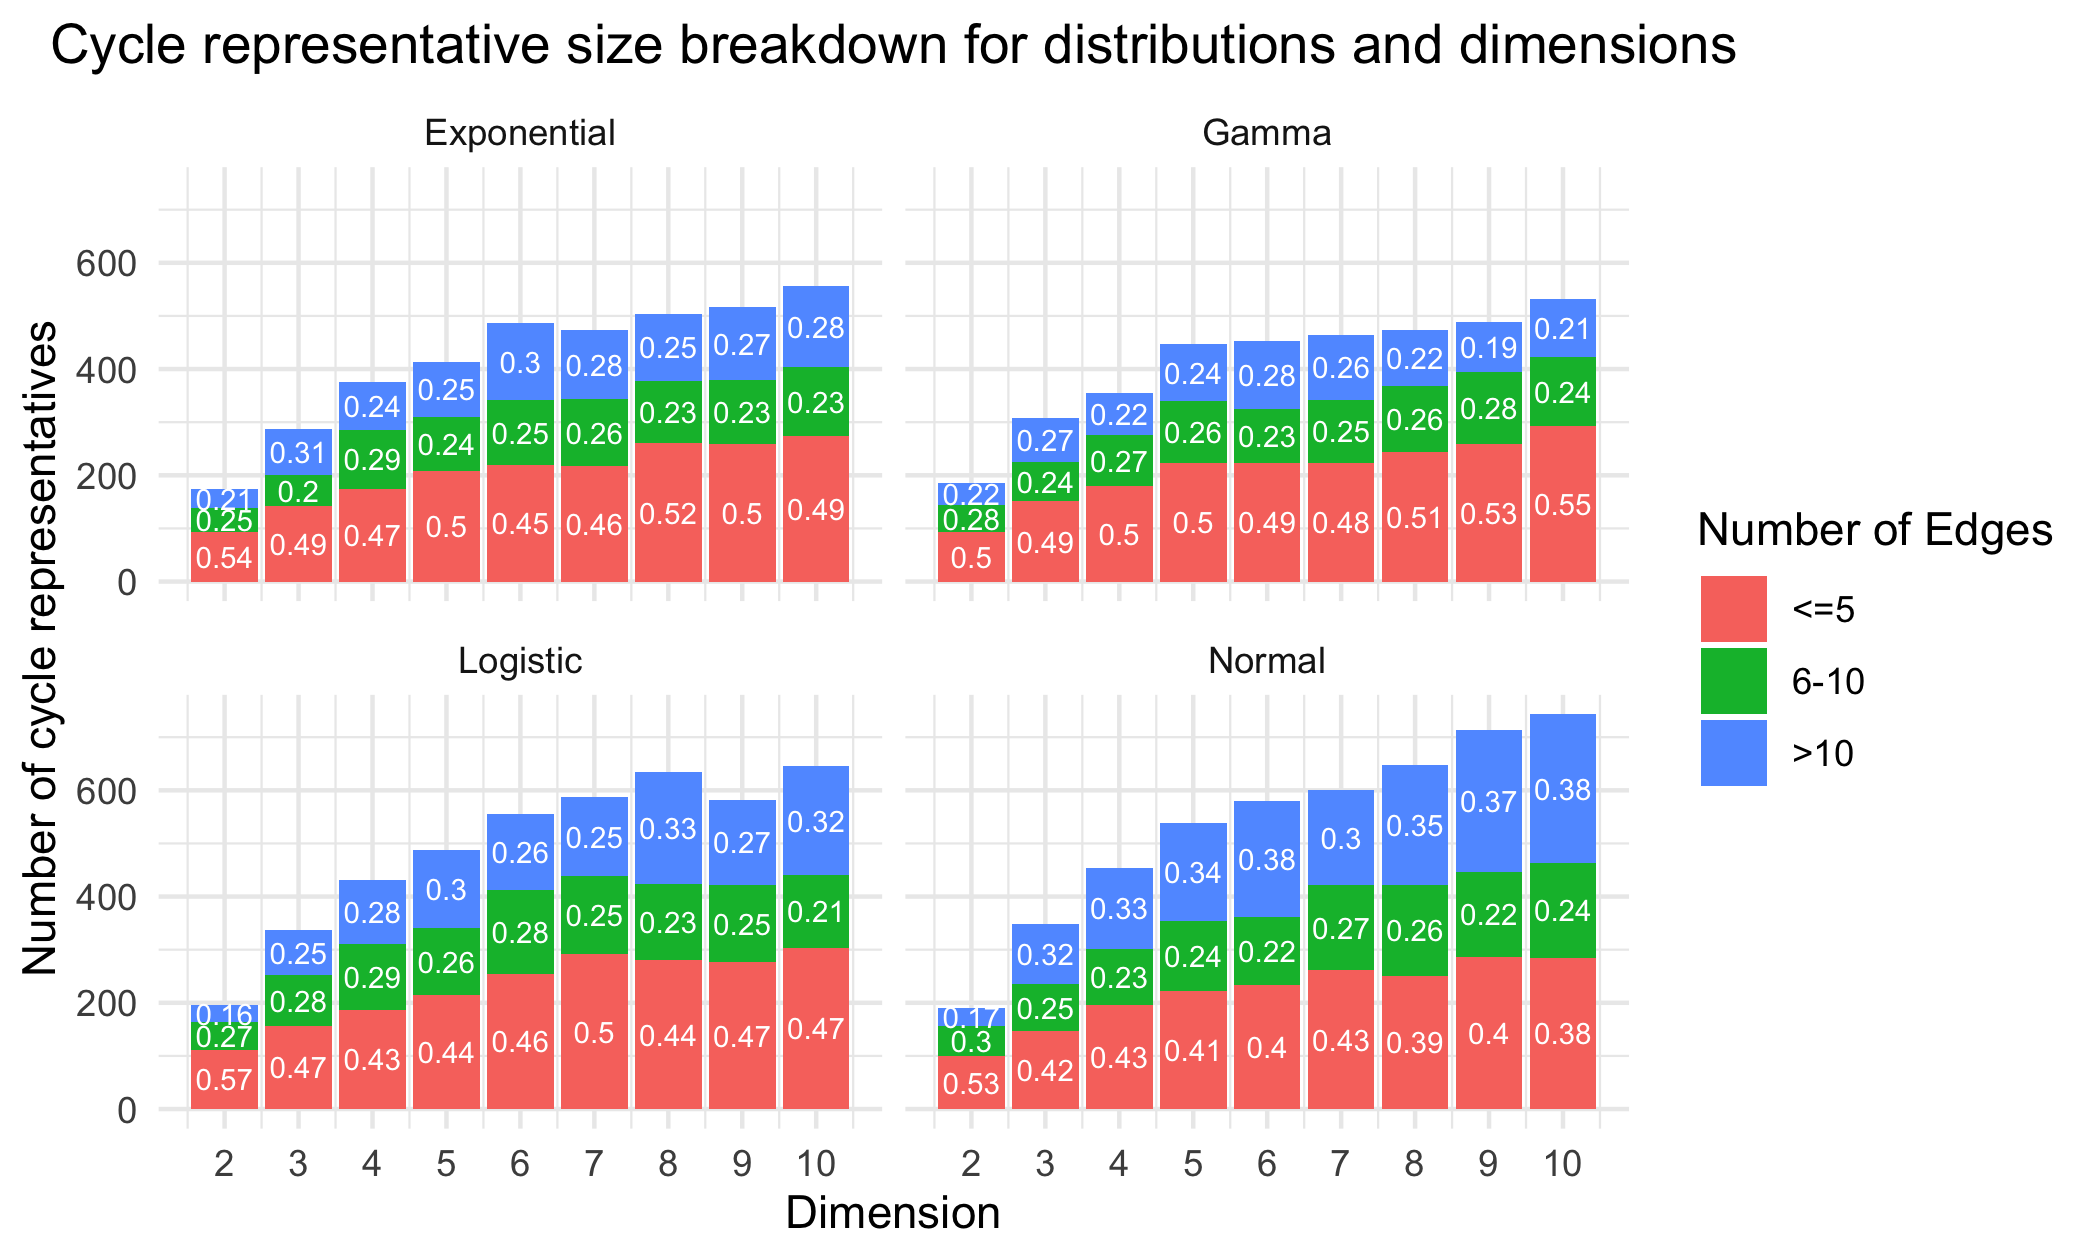
\includegraphics[width=1\textwidth]{figures/generator_breakdown.png}% This is a *.eps file
\end{center}
\caption{The number of original cycle representatives and the number of edges within each original representative for data described in \se \ref{sec: randompointclouds}. These plots aggregate all cycle representatives for each dimension of a particular distribution. The horizontal axis for each subplot is the dimension of the data set, and the vertical axis is the number of cycle representatives found in each dimension. In general, we see there are more cycle representatives in higher dimensional data sets. Each bar is partitioned by the number of edges of the representative. We observe that as dimension increases, there tend to be more cycle representatives with more edges. %\LL{updated 0314}
}\label{fig:gen_num_breakdown}
\end{figure}